\documentclass[sigconf,anonymous,natbib=false,10pt]{acmart}
\settopmatter{printacmref=false}
\setcopyright{none}
\renewcommand\footnotetextcopyrightpermission[1]{}

\acmConference[TBD]{Unclear what}{Sometime
2026}{Somewhere, Earth}


% to be able to draw some self-contained figs
\usepackage{tikz}
\usepackage{amsmath}
\usepackage{hyperref}
\usepackage[normalem]{ulem}
\usepackage{listings}
\usepackage{xspace}
\usepackage{booktabs}
\usepackage{multirow}
\usepackage{wasysym}
\usepackage{caption}
\usepackage{subcaption}
\usepackage{enumitem}
\usepackage[utf8]{inputenc}
\usepackage[compact, small]{titlesec}
\usepackage{algorithm}
\usepackage{algpseudocode}

\captionsetup{labelfont=bf,textfont=rm,belowskip=-8pt,aboveskip=4pt}

% BibLaTeX for bibliography
\usepackage[
  backend=biber,
  style=numeric-comp,
  minalphanames=3,
  isbn=false,
  sortcites=true,
  sorting=anyt,
  abbreviate=false,
  url=false,
  doi=false,
  maxnames=99,
  minbibnames=3,
  maxbibnames=99]{biblatex}
\addbibresource{paper.bib}

\AtBeginBibliography{\small}
\setcounter{biburllcpenalty}{7000}
\setcounter{biburlucpenalty}{8000}

\newcommand{\schedidle}{\texttt{sched\_idle}}
\newcommand{\schednormal}{\texttt{sched\_normal}}
\newcommand{\cgroups}{\texttt{cgroups}}

\newcommand{\eg}{{e.g.},\xspace}
\newcommand{\ie}{{i.e.},\xspace}

\newcommand\hmng[1]{\textcolor{blue!40!red}{[hmng: {#1}]}}

\newcommand{\one}{({\em i}\/)}
\newcommand{\two}{({\em ii}\/)}
\newcommand{\three}{({\em iii}\/)}
\newcommand{\four}{({\em iv}\/)}
\newcommand{\five}{({\em v}\/)}
\newcommand{\six}{({\em vi}\/)}

\def\Snospace~{\S{}}
\def\sectionautorefname{\Snospace}
\def\subsectionautorefname{\Snospace}

\definecolor{codegreen}{rgb}{0,0.4,0}
\definecolor{codegray}{rgb}{0.5,0.5,0.5}
\definecolor{codepurple}{rgb}{0.58,0,0.82}
\definecolor{backcolour}{rgb}{0.95,0.95,0.92}

\lstdefinestyle{rust}{
    %backgroundcolor=\color{backcolour},
    commentstyle=\color{codegreen},
    keywordstyle=\color{codepurple},
    stringstyle=\color{blue},
    basicstyle=\ttfamily\scriptsize,
    breakatwhitespace=false,
    breaklines=true,
    captionpos=b,
    keepspaces=true,
    showspaces=false,
    showstringspaces=false,
    showtabs=false,
    tabsize=2
}
\lstset{style=rust}

%-------------------------------------------------------------------------------
\begin{document}
%-------------------------------------------------------------------------------

%don't want date printed
\date{}

%%
%% The "title" command has an optional parameter,
%% allowing the author to define a "short title" to be used in page headers.
% make title bold and 14 pt font (Latex default is non-bold, 16 pt)
\title{Isolating latency critical from best effort workloads in Linux}

%%
%% The "author" command and its associated commands are used to define
%% the authors and their affiliations.
%% Of note is the shared affiliation of the first two authors, and the
%% "authornote" and "authornotemark" commands
%% used to denote shared contribution to the research.

\author{
{\rm Anonymous Authors}\\
} % end author

%\author{Hannah Gross}
%\affiliation{%
  %\institution{MIT}
%\email{hannah@csail.mit.edu}
%\affiliation{%
%  \institution{MIT}
%  \state{}
  %\country{}
%}

\maketitle

\begin{abstract}
    
Widely-used container orchestration systems like Kubernetes are surprisingly
unable to honor the reservations of LC applications in the presence BE
workloads: a Kubernetes web application's mean latency jumps from 6.2ms to
$\sim$13ms after starting a BE image resize job. This paper traces this problem
down to Linux's cgroups, and show that because Linux uses per-core runqueues,
its weight-based interface is not enforced across cores.

This paper proposes an API that separates best effort workloads from critical
ones with reservations by introducing the BeClass priority class. BeClass
requires fewer cross-core interactions than a weight-based approach, and ensures
that no BE is ever running when an LC is queued. During high load this requires
`parking', which enforces that BEs user-space code doesn't run if doing so would
interrupt an LC process, but continues to run kernel-level services for the BE
so that when load goes down it can continue to run.

Experiments with a BeClass implementation in Linux show that BeClass ensures LC
processes' access to their reserved cores, while running BE workloads
opportunistically. When using BeClass in the same Kubernetes experiment, the
application's mean latency stayed stable at 6.2ms even after starting the BE.

\end{abstract}

%-------------------------------------------------------------------------------
\section{Introduction}
\label{s:intro}
%-------------------------------------------------------------------------------

Cloud providers like AWS and Google, as well as deployment management systems
like Kubernetes, allow users to run services by attaching to each an amount of
resources the service will get. This includes compute (a number of vCPUs),
memory, and sometimes network bandwidth~\cite{aws-ec2-resources,
kubernetes-resources}; the resource this work focuses on is CPU. The guarantee
developers get is that the service will have undisturbed access to that amount
of resources.

Enforcing this guanatee is hard. If providers leave the CPUs idle so they are
available when the service needs them, that leads to a utilization problem. The
load on most applications run in the cloud is variable and unpredictable, so to
account for this developers choose the amount of resources to reserve based on
the expected peak load~\cite{borg, nu, overprovision}. This means that services
with reserved resources rarely use the full reservation they asked for. 

What most systems do instead is allow other workloads to run opportunistically
on temporarly unutilized resources. This includes so-called \textit{best effort}
workloads, which have no reservations, as well letting services with
reservations temporarily \textit{burst}, meaning use more CPUs than they asked
for. This solves the utilization problem, without requiring compromises on the
guarantees made: services with reservations get access to the CPUs they
requested when desired, while best effort or bursting services can make use of
otherwise idle resources.

Kubernetes follows presicely this model. Services fall into three quality of
service (QOS) classes: \textit{Guaranteed}, which have requests (\ie{}
reservations) as well as limits, \textit{Burstable}, which have requests and no
limits, and \textit{Best Effort}, which have
neither~\cite{kubernetes-pod-qos-types}. Guaranteed services are the last to be
evicted from a node experiencing high load, and give more predictable
performance, whereas the Burstable class allows applications with bursty load to
opportunistically make use of available resources, thereby better utilizing the
resources Kubernetes is running on.

AWS similarly supports both guaranteed- and burstable-style reservations, with
their M and T instance types~\cite{aws-ec2-burstable,aws-ec2-resources}. In this
case the motivation for customers to use the burstable-style instance rather
than overprovisioning on guaranteed-style is pricing.


\begin{figure}[t]
    \centering
    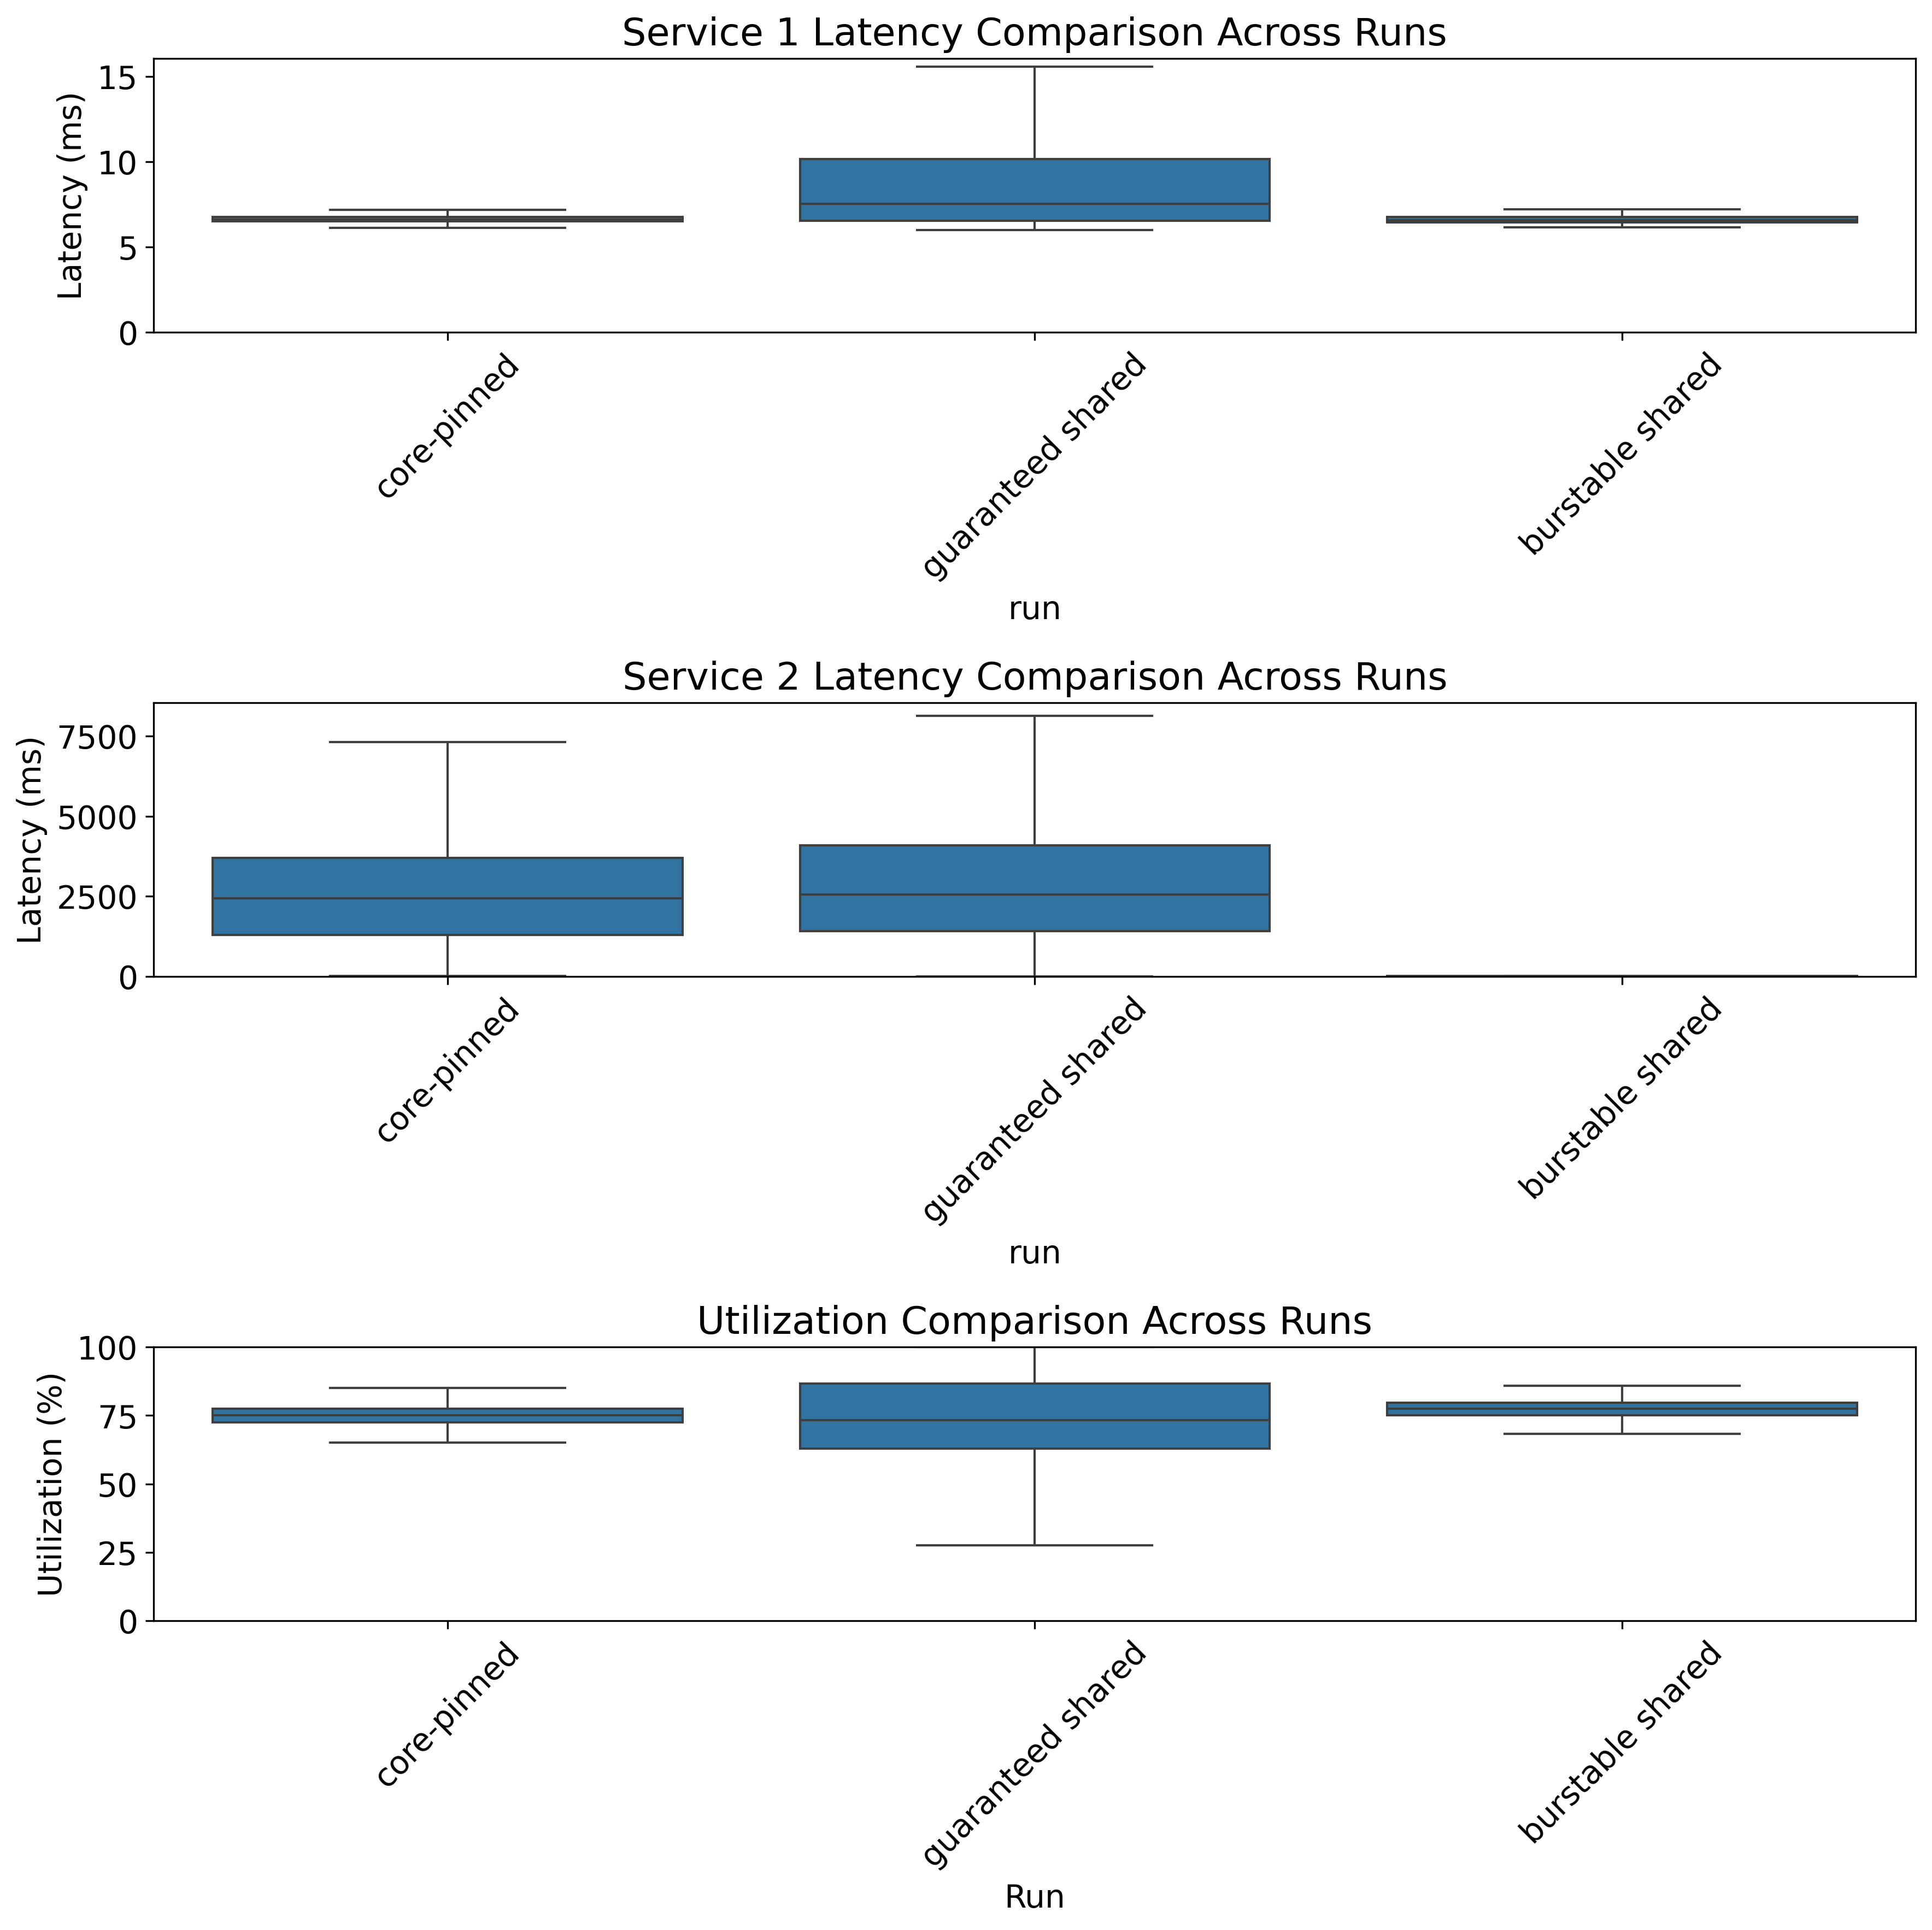
\includegraphics[width=\columnwidth]{graphs/kubernetes-lc-lc-cmp.png}
    \caption{In Kubernetes, running anything alongside a server in the
    Guaranteed QOS class affects the server's
    performance}\label{fig:kubernetes-qos-cmp}
\end{figure}

However, we find that current popular scheduling systems fail to properly
enforce reservations. We use as a case study a small but realistic social
network web application, which we run using Kubernetes.
\autoref{fig:kubernetes-qos-cmp} shows that running anything, even another
guaranteed service, alongside the web server affected its end-to-end latencies,
and that these effects go away when using core-pinning.\hmng{edited up to here}

Understanding why Kubernetes fails to honor the web application's reservation
requires looking at the underlying mechanism enforcing the CPU reservation:
Linux's \cgroups{}. In fact, most modern containers rely on \cgroups{} for CPU
isolation: all Open Container Initiative (OCI) compliant containers, including
Kubernetes but also Docker, CRI-O, and containerd
do~\cite{oci-cgroups,docker-docs-cgroups,container-isolation-article}. VM
frameworks, including Firecracker, AFaas and libvirt, also rely on \cgroups{} to
manage CPU time reservation~\cite{firecracker-cgroups,afaas,libvirt-cgroups}.

Weight is the part of the \cgroups{} interface these systems use for enforcing
the reservations LC applications have, while still allowing BEs without
reservations to run opportunistically.\footnote{Other operating systems expose a
similar interface, for instance Windows exposes a number of shares.} Kubernetes
creates one top level group for all best effort services, called
\texttt{kubepods-besteffort}, inside which all BE pods are placed, and assigns
it the lowest possible weight of 1. Pods with reservations are separated into
Burstable and Guaranteed, the main difference being that Guaranteed pods require
a limit to be set on the resources it can use. Kubernetes calculates the weight
that each pod gets based on the amount of milliCPUs it requests. For instance,
in the \autoref{fig:kubernetes-unedited} experiment, the web application service
ran in the Guaranteed class and asked for 4 CPUs, and Kubernetes assigned the
underlying pod a weight of 157.

The \cgroups{} documentation specifies that each group should get CPU time
proportional to its weight as a share of the sum of weights of runnable
groups~\cite{cgroups-kerneldocs}. However, the latency increase we see after
starting the best effort tasks in \autoref{fig:kubernetes-unedited} is much more
than the 1\% CPU time the server should be losing out on based on its weight. As
we show in more detail in \autoref{s:problem}, the problem that leads to the
increased latencies observed is that Linux will run a low weight process on one
core, unaware that a high weight process is runnable and waiting on another.
This happens because Linux uses per-CPU runqueues, which avoids the overheads of
having a global runqueue. A key challenge this work addresses is managing this
tension between how often the scheduler has to look at all the other cores'
runqueues to enforce reserved processes' priority globally, while still running
best effort ones opportunistically.

Our approach addresses this challenge by creating a new priority class for best
effort tasks to run in, \beclass{}, and enforcing it in the scheduler via
priority scheduling. Linux already has other classes between which it enforces
strict priority, which are designed and used for real time applications
(\autoref{ss:approach:linux-classes-isolate}); the proposed \beclass{} sits
below the default scheduling class. As we show in
\autoref{ss:approach:solves-problems}, putting best effort processes in a
separate class from those with reservations makes it viable to enforce those
reservations across cores, because it reduces the number of times the scheduler
is required to look at all the other cores' runqueues. Enforcing weights across
cores requires the scheduler to do so every scheduling tick, but with a separate
class it only has to look at other cores on \textit{class boundary crossings}:
every time a core switches from running an LC process to running a BE on, and
every time it enqueues an LC process.

A challenge with creating a separate priority class arises when the LC class is
under high load: completely starving best effort processes can lead to issues
such as deadlocks, broken TCP connections, or missed timers. The goal is to make
the priority of processes with reservations over those without as strict as
possible, while still allowing BE processes to resume execution normally once
the load goes down, even if the high load lasts for multiple minutes.

We address this challenge by enabling best effort processes to exist in an
ephemeral state called \textit{parked}, which they enter when the CPU
utilization is high enough that processes with a reservation account for all the
CPU time. While load remains high, the scheduler ensures that the parked BE's
user-space process doesn't run and consume resources, but continues to run the
kernel-space handlers that manage critical state, including TCP connections and
timers, on behalf of the BE processes. 

We implement \beclass{} in Linux on top of an existing scheduling policy called
\schedidle{}, and show that it is able to significiantly improve Linux's ability
to honor reservations while sharing CPUs with best effort workloads: in the same
Kubernetes experiment, the increase in average latency when starting a BE
workload goes from $>$2x to 0. The contributions of this paper are thus as
follows: 
\begin{enumerate}
    \item identifying as the reason LC tasks' reservations are often violated is
    that \cgroups{} does a poor job of enforcing the weights across cores;
    \item the design of \beclass{}, a new class for best effort tasks whose goal
    is to enforce reservations in the presence of BE processes by using priority
    scheduling, that reduces the points in time it needs to look at other core's
    runqueues, as well as enforcing the parked state
    \item an implementation of \beclass{} in Linux
\end{enumerate}

%-------------------------------------------------------------------------------
\section{Problem}\label{s:problem}
%-------------------------------------------------------------------------------


\begin{figure}[t]
    \centering
    \begin{subfigure}[b]{0.49\columnwidth}
        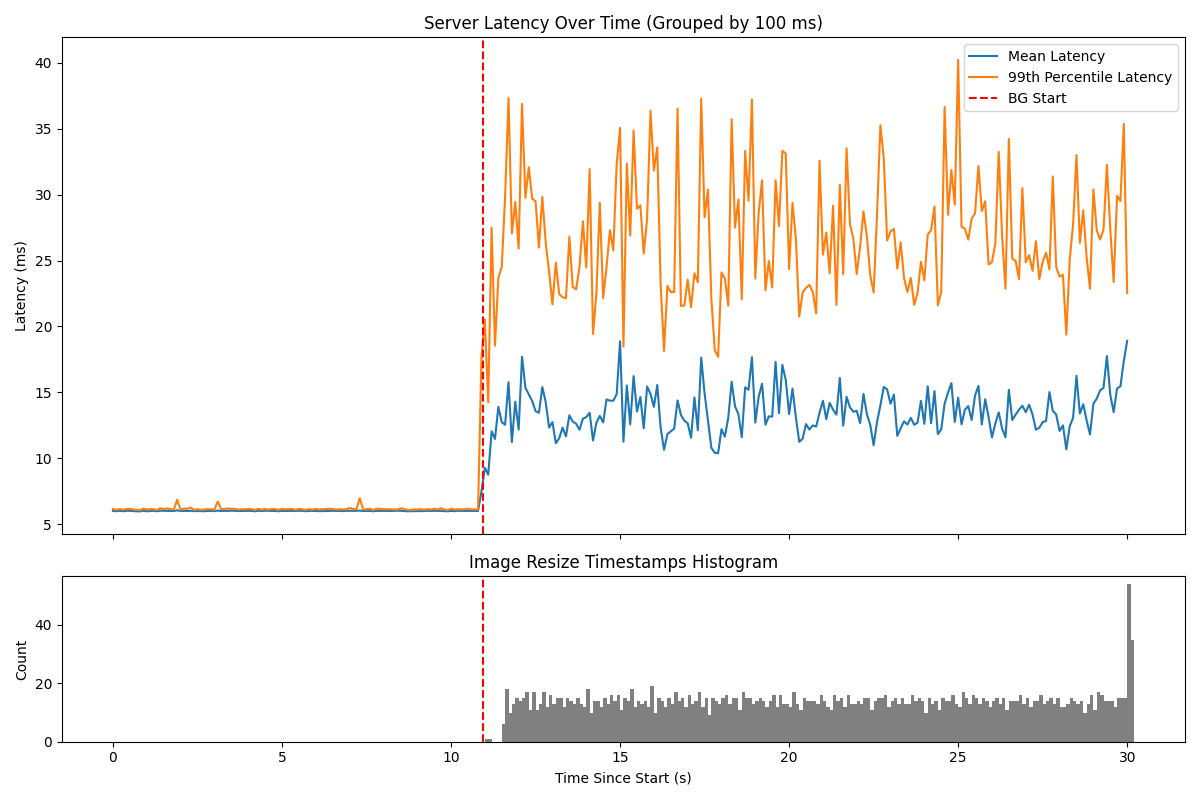
\includegraphics[width=\columnwidth]{graphs/srv-bg-unedited-low.png}
        \caption{Low load stetting, utilization before starting the BE tasks is
        around 85\%}\label{fig:srv-bg-unedited-low}
    \end{subfigure}
    \hspace{\fill}
    \begin{subfigure}[b]{0.49\columnwidth}
        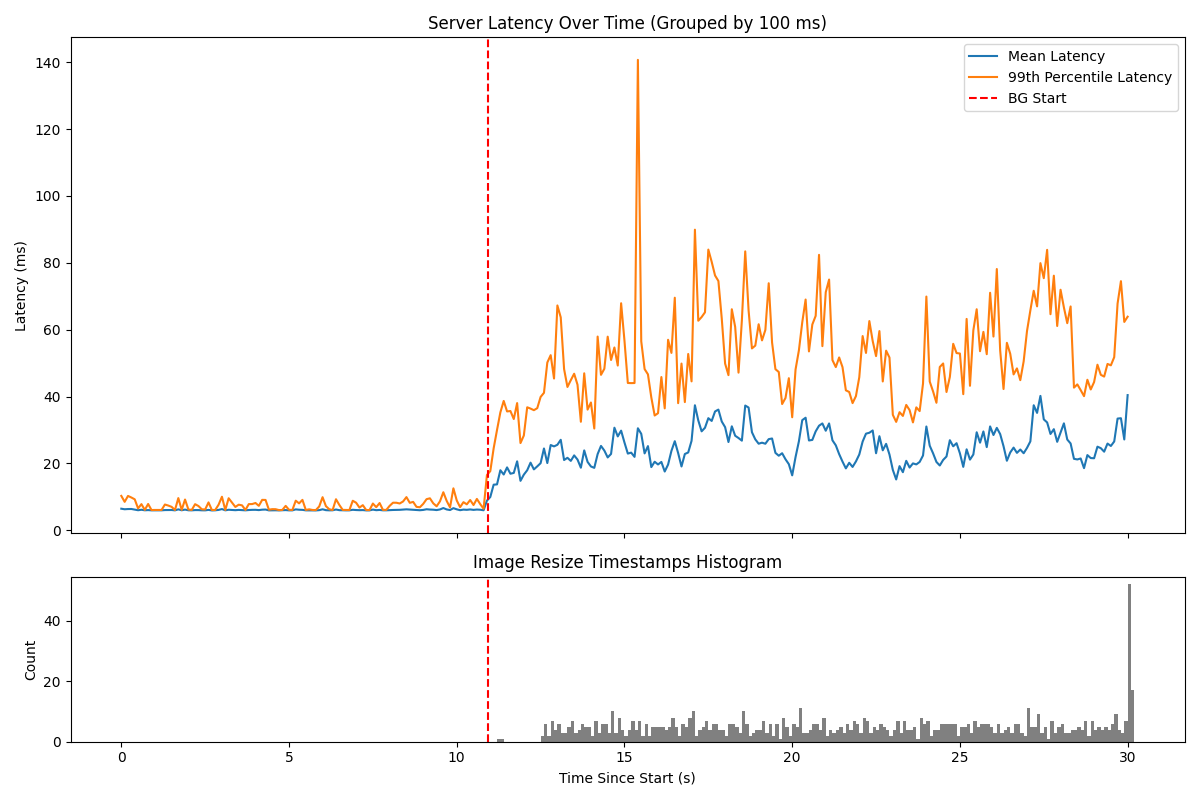
\includegraphics[width=\columnwidth]{graphs/srv-bg-unedited-high.png}
        \caption{High load setting, utilization before starting the BE tasks is
        around 95\%}\label{fig:srv-bg-unedited-high}
    \end{subfigure}
    \vspace{4pt}
    \caption{Latencies of the server and iteration counts of the background
    tasks in different load scenarios. Note the different y axis limits. The
    upper graphs show end-to-end request latencies, and the bottom graph is a
    histogram of completed iterations of the BE tasks}\label{fig:srv-bg-unedited}
\end{figure}

In order to understand more concretely where the isolation between the LC web
application and the BE image resize is failing in
\autoref{fig:kubernetes-unedited}, we reproduce the jump in latency we saw in
the application running on Kubernetes in a simpler benchmark. We run a simple
cpu-bound server with a pool of worker threads that we hit with an open-loop
remote client, and then start two BE workloads doing image resizing. We put the
LC server and the BE resize job each in their own \cgroups{} group, with weights
1 and 10000. \autoref{fig:srv-bg-unedited} shows the increase in latencies of
the LC server at two different baseline utilization levels. We see that even in
the lower baseline utilization case, where the server alone uses 85\%, mean
latencies spike up from steady at around 6ms to as high as 20ms, and much higher
for 99th percentile latencies.

\begin{figure}[t]
    \centering
    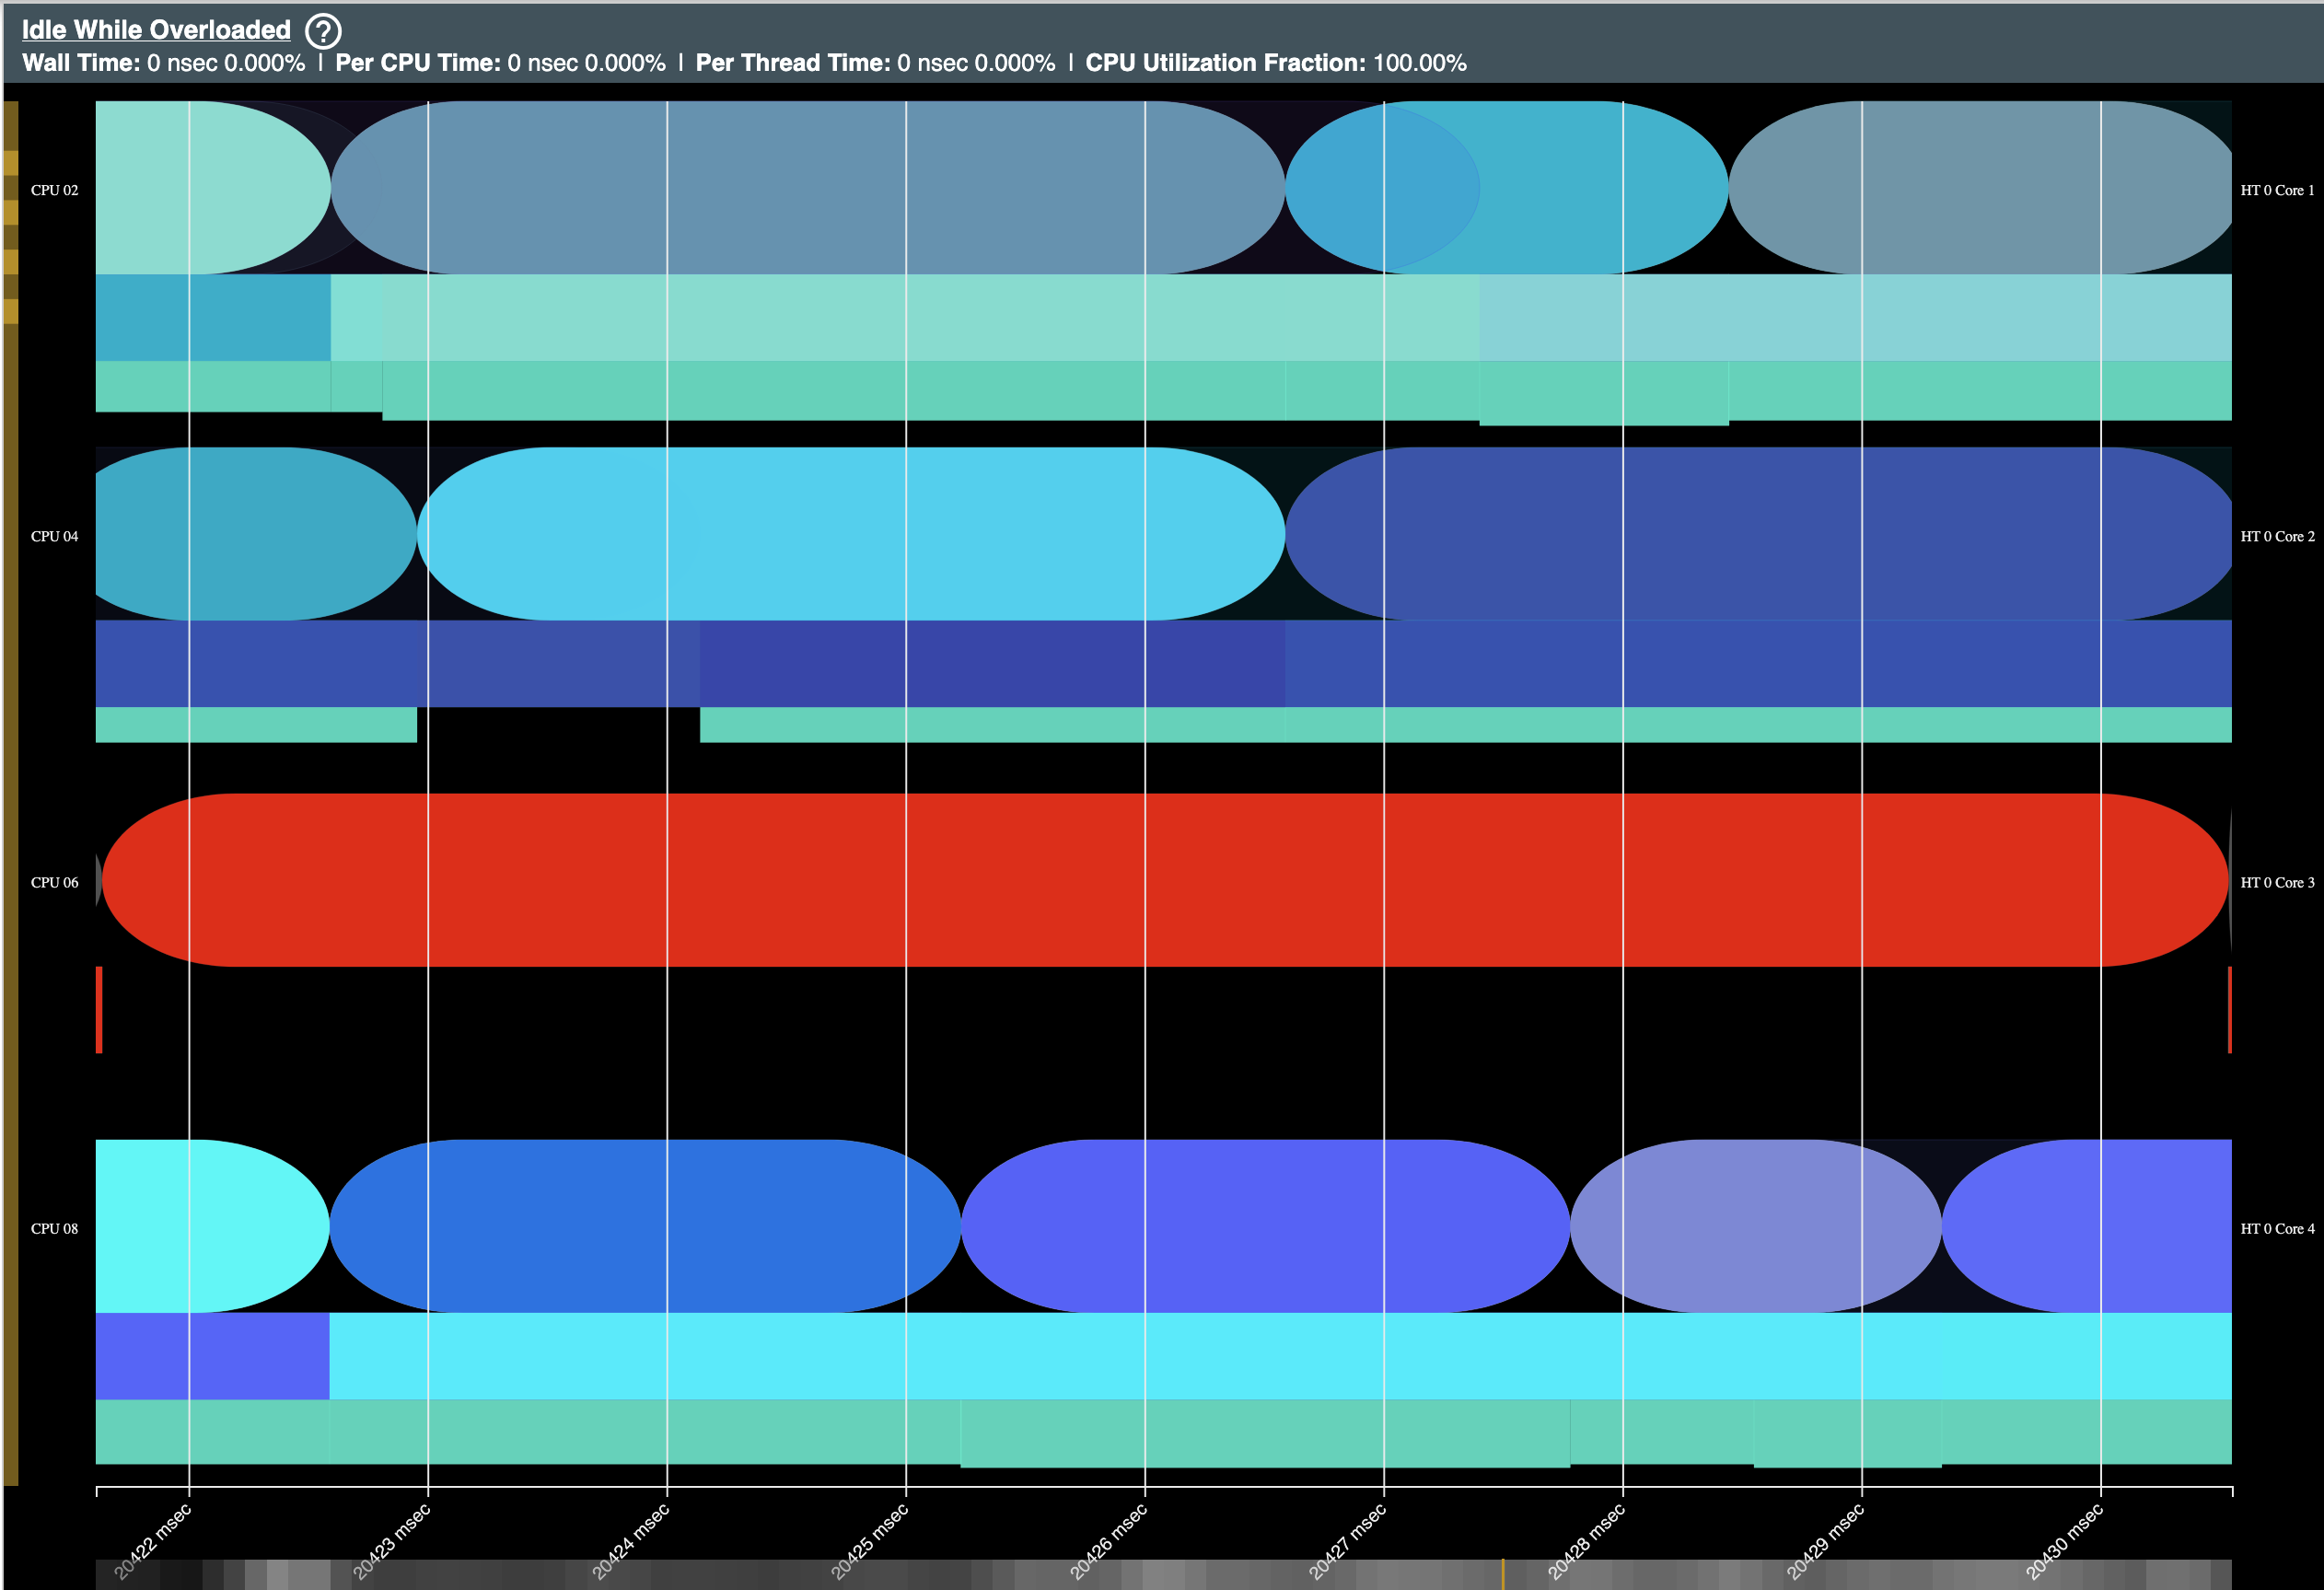
\includegraphics[width=\columnwidth]{graphs/schedviz-problem.png}
    \caption{Each thread is a different color. Circles represent which
    thread is running on that core, while rectangles underneath show waiting but
    runnable threads
    }\label{fig:schedviz-problem}
\end{figure}

Using this simplified experiment, we analyze perf traces of the scheduling
decisions, and visualize the trace using schedviz~\cite{schedviz-tool}, in order
to understand where the latency impact comes from.
\autoref{fig:schedviz-problem} shows a 10ms outtake of the resulting image. The
process running on each core is shown as a an oval, and queued processes are
shown as rectangles below. The root of the undesirable behavior is: on core 6,
the red process that is running the whole time is a BE process, whereas LC
threads, shown in varying shades of blue, are queued on the other cores. The
takeaway here is that the failure mode we observe is that \textit{one core is
running a BE process, while an LC process is waiting on another}.

Based on this observation, we explore more deeply the root of the issue that is
causing the poor behavior we see.

\subsection{Weights are only enforced locally}\label{ss:problem:mechanistic}

The reason this happens is that Linux maintains a separate runqueue on each
core, in order to avoid the synchronization overheads of accessing global state
for every scheduling decision. Within each runqueue, Linux's scheduler works to
maintain the correct ratio of received CPU time at each scheduling; but Linux
does not enforce the weight ratios across cores. This leads to the above failure
mode, where one core has no runnable high weight processes and thus runs a low
weight one, whereas another core has queued high weight processes. This problem
goes away when there are no BE processes, because cores try to steal work before
going idle.

\subsection{Enforcing weights across cores is
expensive}\label{ss:problem:cross-core-hard}

The root of the problem goes deeper than just a poor implementation: a
weight-based interface is at odds with machine-wide policy enforcement. In order
to strictly and globally enforce a processes weight, the scheduler would need to
synchronize at every scheduling decision: calculating whether a given process is
owed time globally requires knowing the total weight across all cores as well as
the sum of time that all the processes in the group have gotten. In increasingly
multi-core and multi-NUMA machines, synchronization is expensive; other work has
found that kernel lock contention is a bottleneck to performance at
scale.~\cite{afaas} This means that the overheads of maintaining global
invariants can quickly become prohibitive.


\subsection{Weights interact poorly with tick-based
scheduling}\label{ss:problem:quantum}

Even on a single runqueue, using very large weight differentials as an interface
to isolate LC and BE doesn't work well because preemption is tick-based. In a
weight based scheme, BE processes also get a fair share of the CPU. The problem
is that, when this happens, the BE process will interrupt any running LC process
for a whole tick. In Linux, hardware ticks are 4ms long. This means that an LC
thread processing a request may be interrupted for up to 4ms, provided the BE
process runs for that long before blocking. 4ms can be a large amount of time
for microservice workloads, whose SLOs are often in the low double digit or even
single digit ms realm.~\cite{sigmaos}




\section{Approach \& Uniqueness}

In order to enforce reservations while running BE jobs opportunistically, our
approach uses priority scheduling instead of weights.

Enforcing priorities requires fewer global runqueue searches than weights do,
because they only need to happen on \textit{class boundary crossings}: on
\exit{}, when a core switches to running lower class processes after having
previously been running high class, and on \entry{}, when a core enqueues a high
class process. These checks ensure that a core $c$ running a BE thread $t$ knows
that there are no queued LC threads anywhere: the \exit{} check ensures theres
none when starting to run $t$, and the \entry{} check ensures if one wake up
while running $t$ it will interrupt $t$.

\begin{figure}[t]
    \centering
    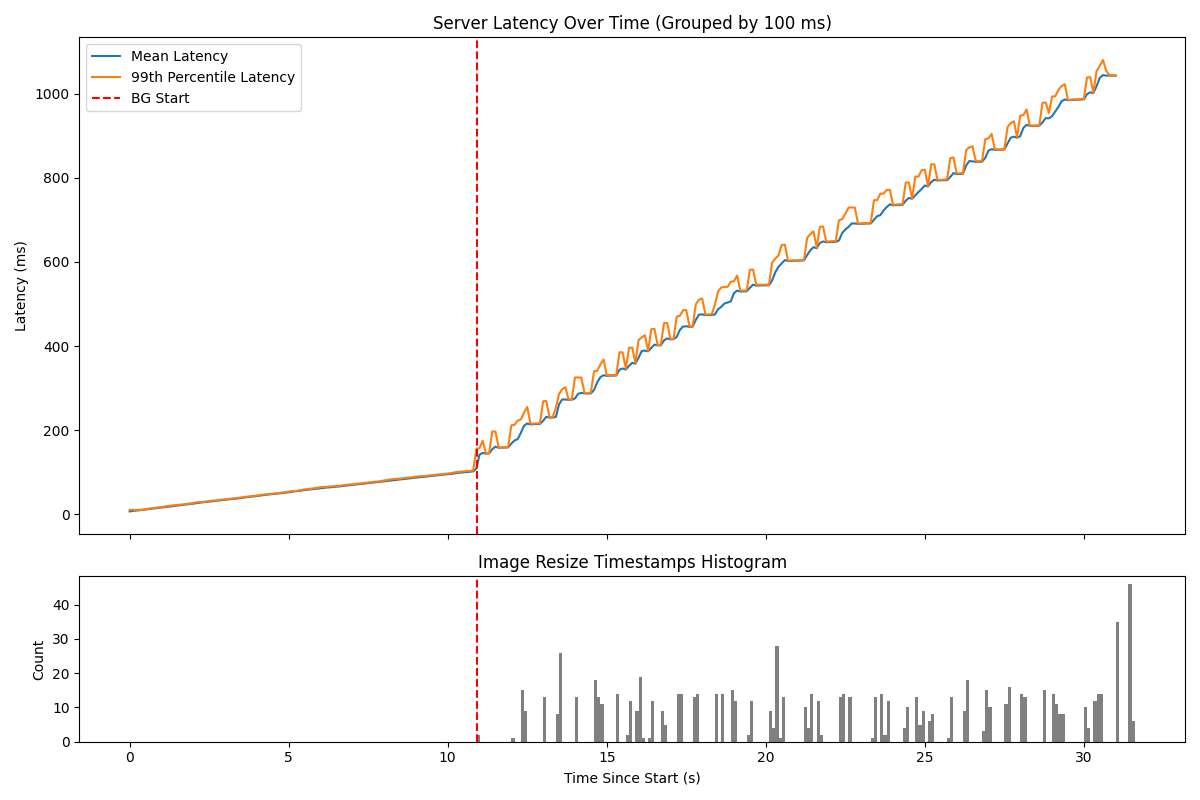
\includegraphics[width=\columnwidth]{graphs/overload-rt.png}
    \caption{when running the server in real time, throttling degrades
    its performance at high load}\label{fig:overload-rt}
\end{figure}


Linux already provides priority scheduling across scheduling classes, but it is
designed for real time applications: if these experience high load, Linux
throttles them in order to not starve the default class. We can see this
happening in \autoref{fig:overload-rt}, where throttling leads to spikes in the
BE task's throughput, and corresponding spikes in the server's latency.

We design a new scheduling class \beclass{} that sits at a lower priority than
\normalclass{}, which enforces LC applications' uncontended access to CPUs they
reserved. To enforce reservations under high load, without throttling the LCs or
killing the BEs, \beclass{} \textit{parks} BE processes, meaning the user-space
code never runs, only kernel-level services.
% \section{Solution}\label{s:solution}

\hmng{currently working on this; her structure is in fl ux but most of the main
ideas are in there? }

The performance of the current \schedidle{} policy shows us that if we want to
completely isolate LC and BE, we need to put BE in a an entirely separate
scheduling class.

Linux has a strong requirement for fairness in its scheduling: even though there
are strict priorities between the scheduling classes, Linux ensures that
Deadline and Fifo processes can never starve Normal ones, by rate-limiting each.
And within the Normal scheduling class the approach is to insluate processes
from each other by using weighted fair share scheduling, not priorities.

For the Deadline class this is fine because it does admission control so there
is never unexpected throttling. For the Fifo class the rate-limiting may lead to
throttling, but it is expected that the realtime applications encompass a small
set of high-sensitivity and low-processing-time workloads. As such, the Fifo
class is not expected to reach high utilization except in error.

However, it is expected that LC processes temporarily use all the
available cputime. We argue that LC tasks should not ever be throttled to run BE
tasks, especially in a system like Linux where the interruption could
potentially last a full scheduling tick. 


\subsection{The case against fair scheduling}


An alternative would be to simply enforce the weights properly across cores.
This is an unappealing proposition for two main reasons: (1) small weights are
still weights, and (2) enforcing a split across cores requires more
syncronization than enforcing a strict priority.

Although low weights run infrequently, they still get a fair share, and in doing
so impact the latency of the higher weight (LC) processes. As we argued in
section \autoref{s:why}, a large number of BE workloads each with a small weight
could add up to represent a significant amount of weight in the system, now
contending directly with the LC workload. Weights also interact with the 4ms
tick granularity unfortunately, where when it is a low-weight processes time to
run, it will likely be scheduled for a full tick. It is common for microservices
to have SLAs in the order of 10ms or even less, where a gap of 4ms will have a
significant impact on response latency. Compounded with a large number of BE
workloads, this can lead to significant overheads even in a world where weights
are correctly enforced across cores.




\subsection{The case for unfair scheduling}


If it is the case that the starvation lasts a long time (more than the expected
load burst duration, on the order of milliseconds), then that is a distributed
scheduler's problem, and needs to be solved at a distributed level. In the mean
time, we argue that that machine should continue to run the LC tasks as fast as
it can. We explore the implications of starving for more extended periods of
time (order of tens of seconds) in the evaluation.\hmng{this argumentation feels
more from first principle than I think you'll like, and could be better
organized }



\section{Implementation}\label{s:implementation}

A categorical differentiation in the scheduler allows for fewer synchronization
points without compromising the enforcement of global isolation. In order to
enforce a categorical priority, the scheduler only needs to sychronize at two
points: on \textit{entry}, when a new high-priority thread wakes up on a core
already running something high-priority, and \textit{exit}, when starting to run
a low priority thread. If on entry the scheduler looks for cores running low
priority work to go interrupt, and on exit the scheduler looks for high priority
work to steal, it has ensured the global property that \textit{no core is ever
running a BE process while an LC one is runnable and waiting}.

In order to affect the changes required, we modify Linux and put in the pieces
to make \schedidle{} effectively its own scheduling class. We chose to do this
rather than create an entirely new scheduling class in the code, which would be
intellectually cleaner and closer to the conceptual reality, but would require
more code changes and leave \schedidle{} in it's current half-formed
state.

We patch Linux version 6.14.2, and the patch requires XX lins of code change. It
intervenes in two places in the current scheduling process of the Normal
scheduler: 
\begin{enumerate}
    \item it ensures that no \schedidle{} entity will be chosen if there is a
runnable \schednormal{} entity (this overrides the fair share that even a weight
1 process would occasionally get in the unmodified kernel),
    \item it tries to steal queued \schednormal{} entities from other cores
before running a \schedidle{} entity.

\end{enumerate}


Doing the first part required changing the code that picks the next entity in
the Normal scheduler, in the function \texttt{pick\_eevdf}. The Normal scheduler
maintains the runqueue in the structure of a binary tree, which is ordered by
the amount of virtual CPU time each process has gotten (virtual because it takes
into account the entities weight). The current function searches that tree, and
chooses the most leftmost eligible entity to run. The patch first adds checks
whether the runqueue is currently in an `idle' state, ie only has \schedidle{}
entites on its runqueue. If that is true then the search is performed as usual,
if not then the patch checks each movement through the tree to ensure that the
subtree being chosen has at least one \schednormal{} entity, and that the final
process chosen is one as well. This ensures that the most eligible
\schednormal{} task is chosen to run next.

Should the task chosen be in \schedidle{}, but the one running before was
\schednormal{}, then we know we are in an \textit{exit} path. The patch adds
code that, in this situation, will try to steal queued \schednormal{} tasks from
other cores. It will steal up to half of the busiest cores' queued
\schednormal{} tasks.


%-------------------------------------------------------------------------------
\section{Evaluation}
\label{s:eval}
%-------------------------------------------------------------------------------

This section answers the following questions:
\begin{enumerate}
    \item Does \schedbe{} isolate LC from BE workloads?
    \item Can parked processes resume correctly? How many resources does it used
    while parked?
    \item How much does \schedbe{} cost?
    \item How does \schedbe{}'s isolation compare to that of \schedidle{}?
\end{enumerate}

All the graphs in this paper run on Linux version 6.14.2, the baseline version
that our implementation builds on.

\subsection{Does \schedbe{} isolate?}

\begin{figure}[t]
    \centering
    \begin{subfigure}{\columnwidth}
        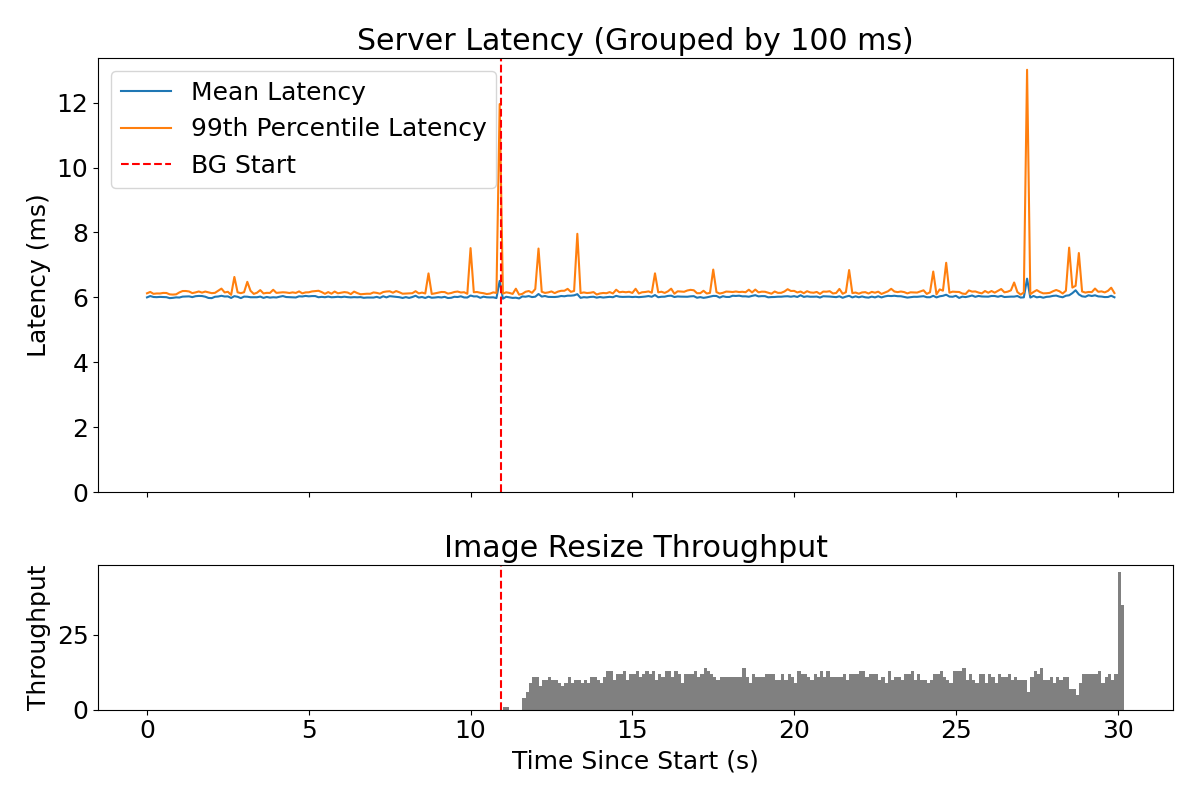
\includegraphics[width=\columnwidth]{graphs/srv-bg-schedbe-low.png}
        \caption{Low load (85\%)}\label{fig:srv-bg-schedbe-low}
        \vspace{12pt}
    \end{subfigure}
    \begin{subfigure}{\columnwidth}
        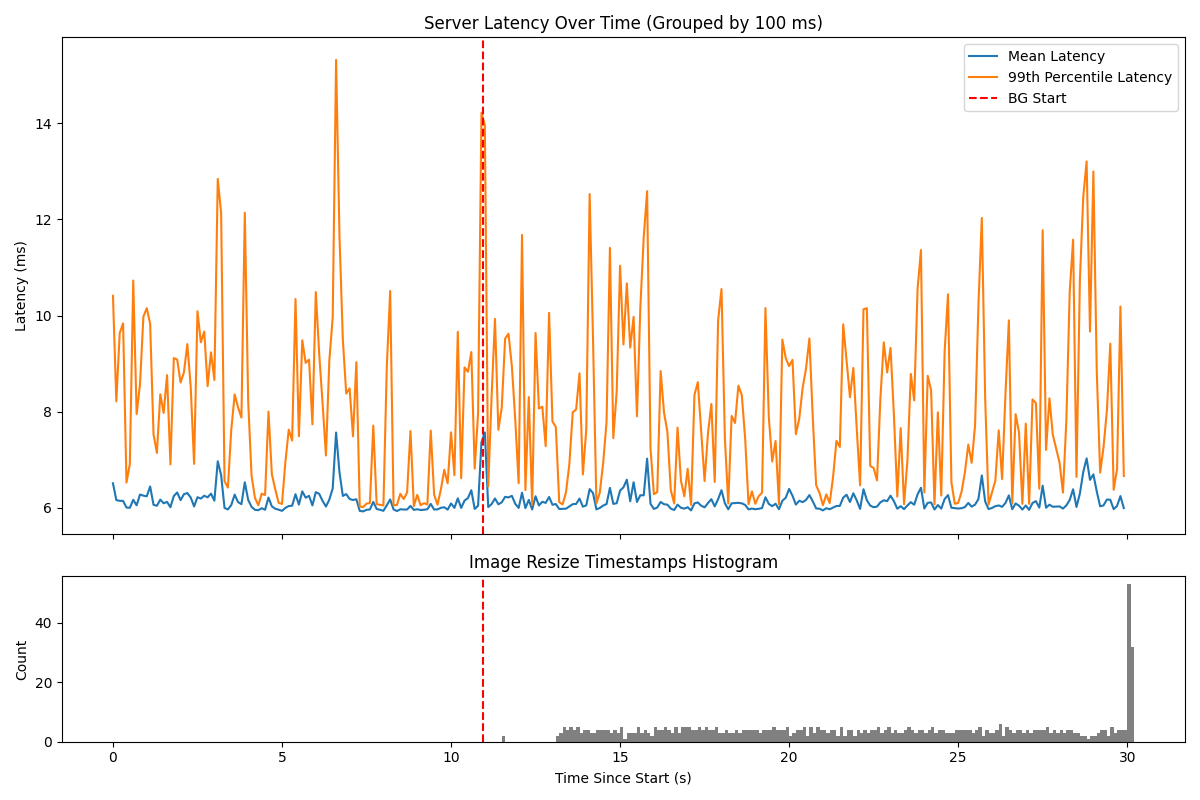
\includegraphics[width=\columnwidth]{graphs/srv-bg-schedbe-high.png}
        \caption{High load (95\%)}\label{fig:srv-bg-schedbe-high}
    \end{subfigure}
    \vspace{4pt}
    \caption{same expiriment as in \autoref{fig:srv-bg-weight-150}, but with the
    BEs running in \schedbe{}}\label{fig:srv-bg-schedbe}
\end{figure}

\begin{figure}[t]
    \centering
    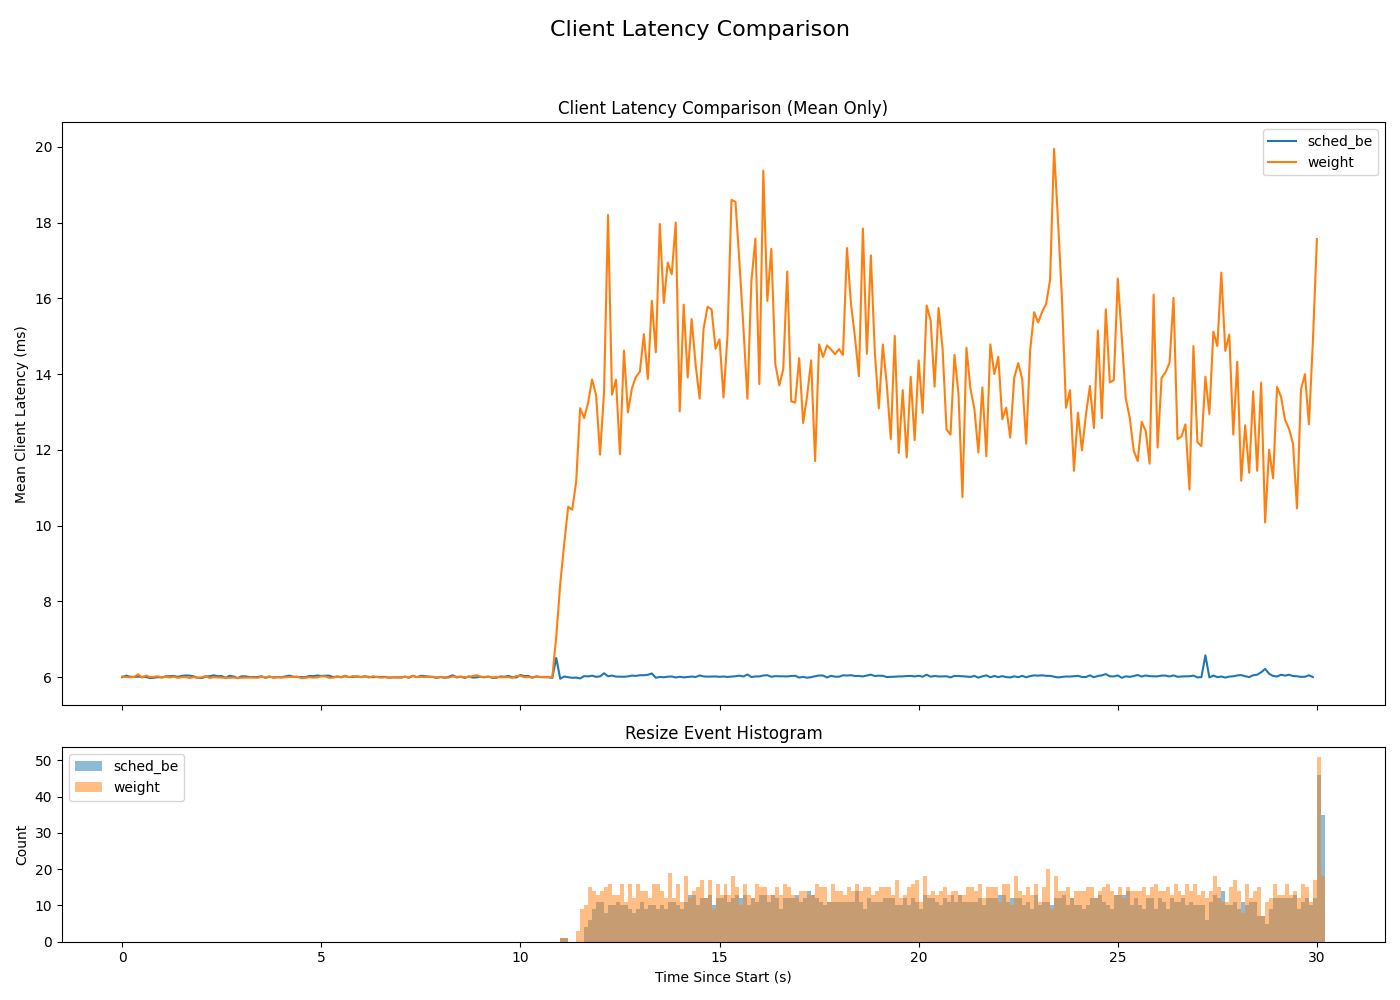
\includegraphics[width=\columnwidth]{graphs/srv-bg-cmp-unedited-schedbe.png}
    \caption{A direct comparison between the server latencies when using the
    existing \cgroups{} weights versus \schedbe{} to isolate the LC from the
    BE}\label{fig:srv-bg-cmp-unedited-schedbe}
\end{figure}

\begin{figure}[t]
    \centering
    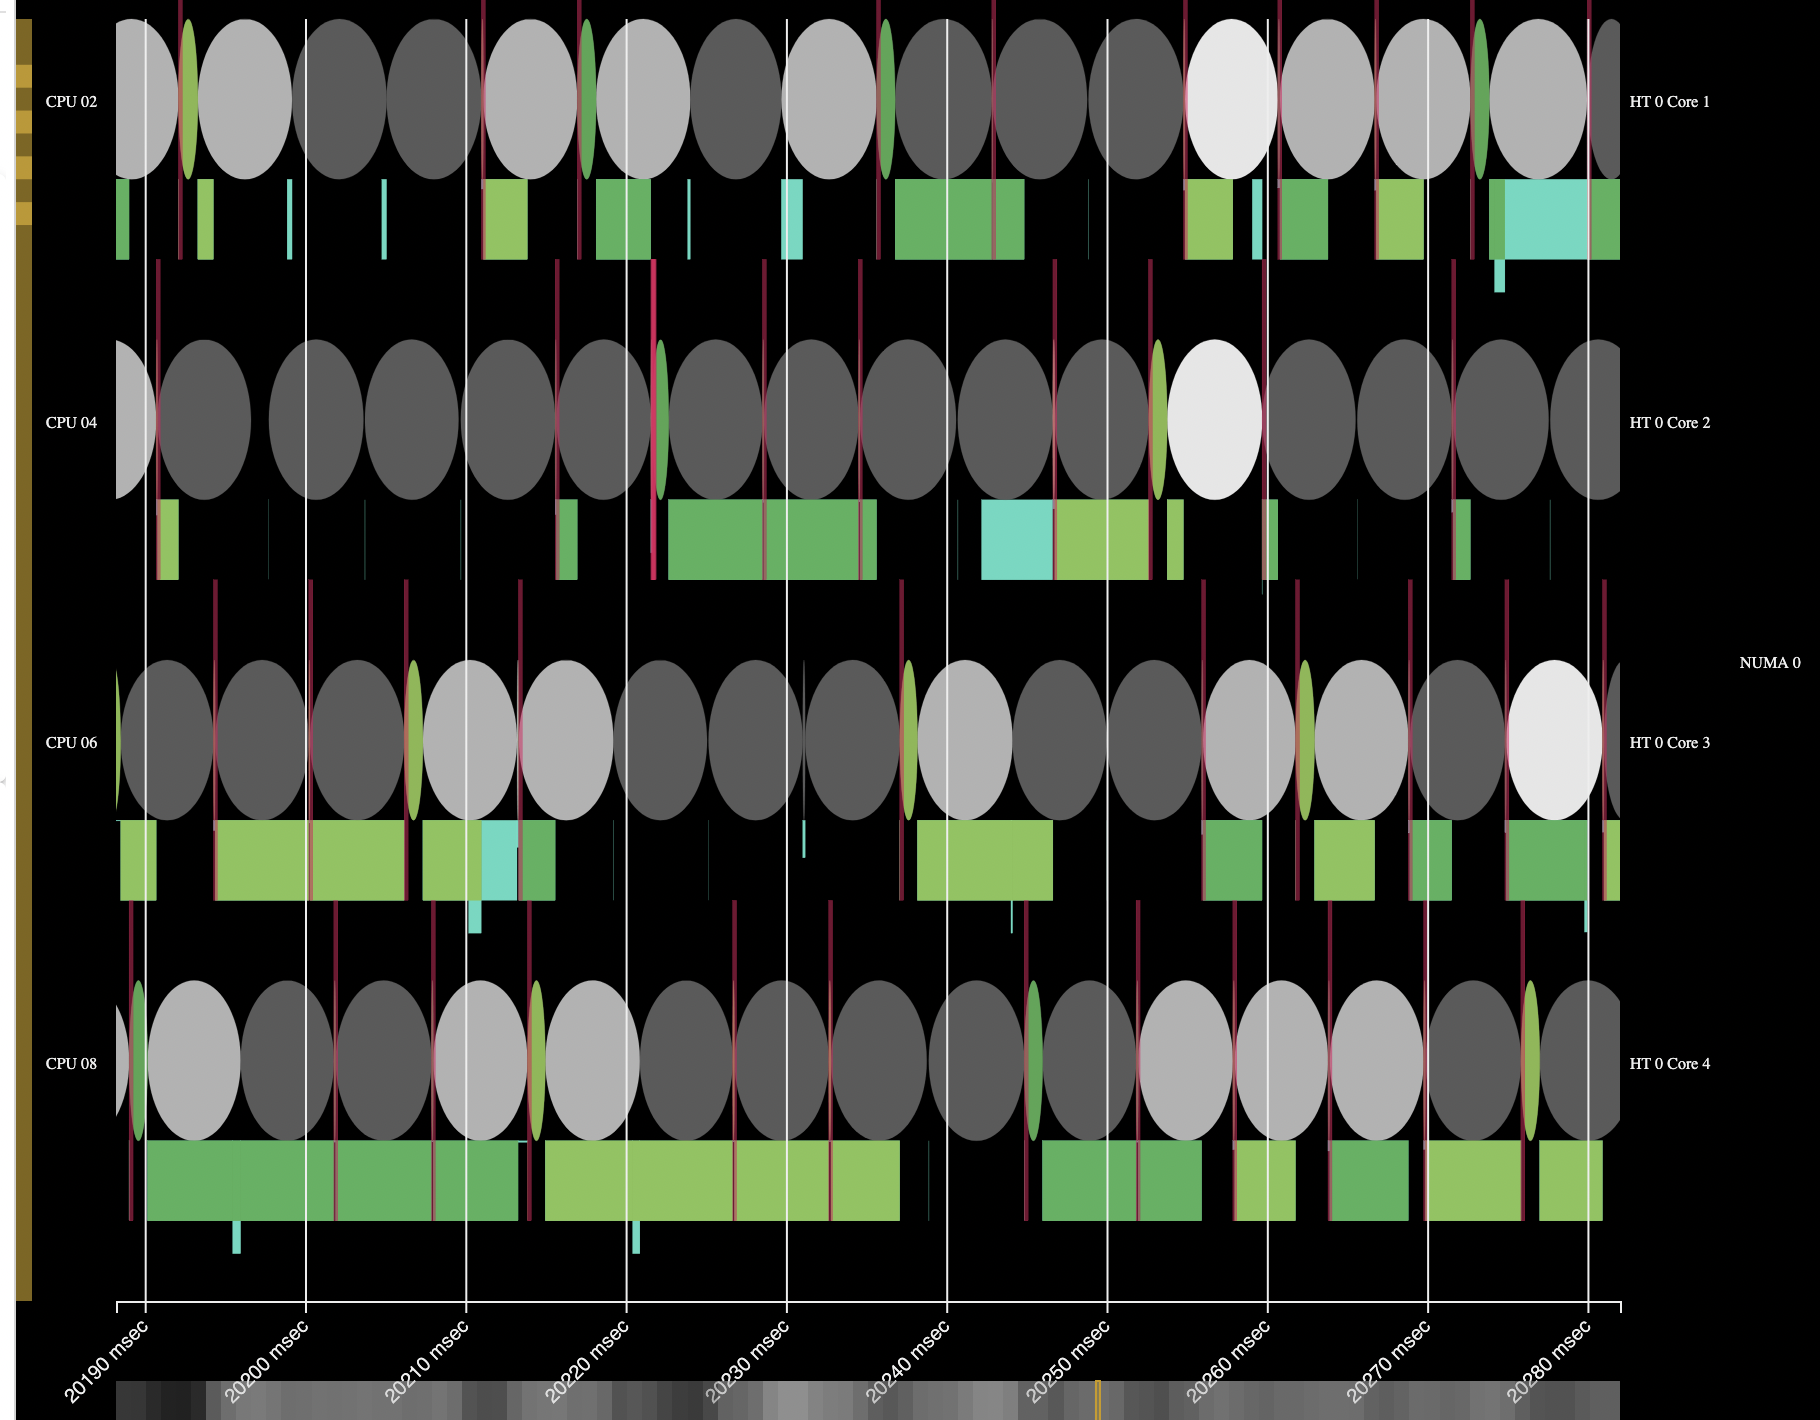
\includegraphics[width=\columnwidth]{graphs/schedviz-schedbe.png}
    \caption{BE threads only run in the gaps when there are no queued LC
    threads. The BE threads are colored in two different shades of green, the LC
    threads are the grey ones (all the threads are the same shade of grey, the
    different shades have to do with the amount of processes the visualizer has
    grouped). The red vertical lines are the scheduler initially choosing a BE
    thread, which leads to an attempt to steal a queued LC one.
    }\label{fig:schedviz-schedbe}
\end{figure}

We run the microbenchmark experiment from \autoref{fig:srv-bg-weight-150} using
\schedbe{}. We can see the resulting performance in
\autoref{fig:srv-bg-schedbe}, and \autoref{fig:srv-bg-cmp-unedited-schedbe}
shows a direct comparison between the original benchmark run on \cgroups{}
weights and running it using \schedbe{}. As desired, the latency of the server
remains stable after the background tasks start. This does not mean that the
background task never runs: the lower part of each graph still shows iterations
of image resizing being done. The difference is that now the background tasks
will reliably get interrupted when the LC server has a request to process.
\autoref{fig:schedviz-schedbe} shows this happening in an outtake of a schedviz
visualization. The green BE processes run only in the gaps where there is no
queued LC process, and are immediately preempted when one wakes up, on whatever
core that may be. The vertical red lines show when the \exit{} path \schedbe{}
introduced runs, \ie{} when the core has chosen intially to run a BE process
after having previously run LC. As we can see, this is sometimes followed by
just running the BE, but often by the core running an LC process, meaning that
it succesfully found and stole a queued and waiting LC thread.

\begin{figure}[t]
    \centering
    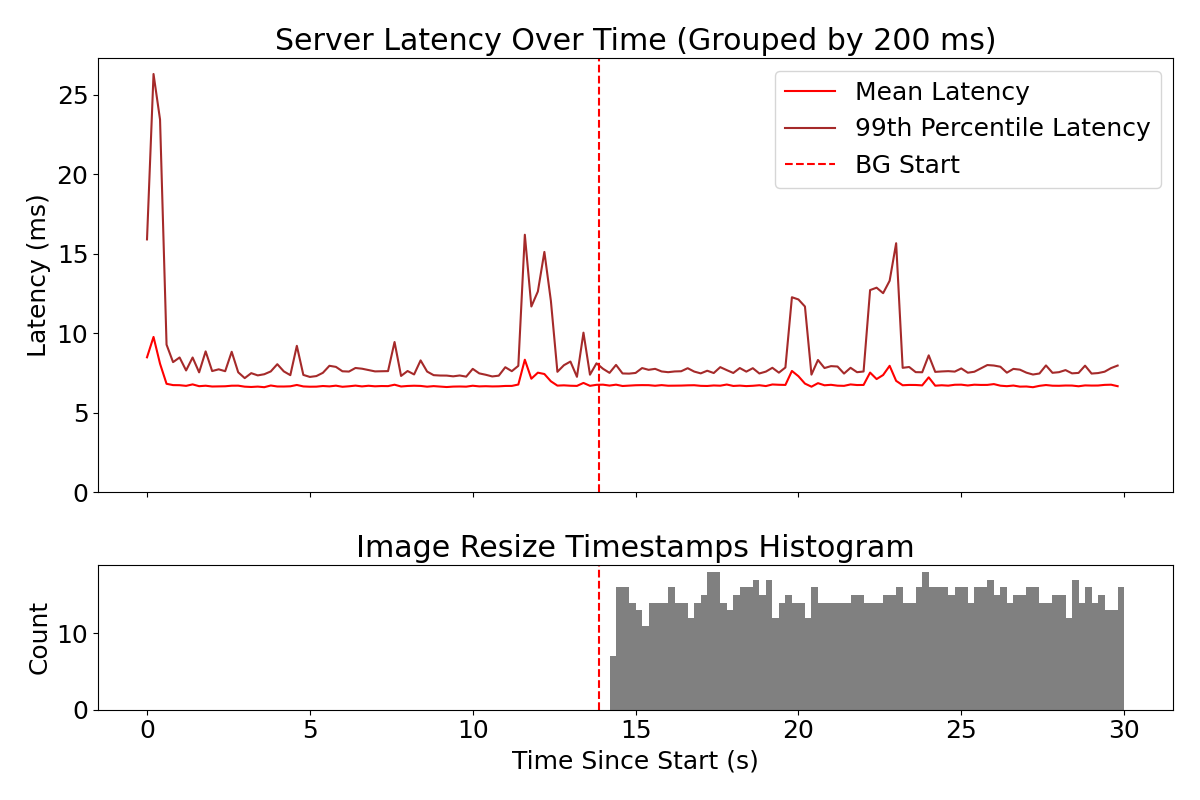
\includegraphics[width=\columnwidth]{graphs/kubernetes-schedbe.png}
    \caption{The same experiment as in \autoref{fig:kubernetes-unedited}, but
    running the BE as a \schedbe{} task}\label{fig:kubernetes-schedbe}
\end{figure}

We also run the Kubernetes application from \autoref{fig:kubernetes-unedited}
using \schedbe{}. The results are in \autoref{fig:kubernetes-schedbe}. We can
see that again the latency profile of the LC web application looks largely the
same before and after starting the image resize job.\hmng{run for longer and/or
get concrete numbers for how much it increases, vague hedging (largely, not
entirely) is not good} It is not entirely without spikes, but the spikes come
from interference with Python runtimes and Kubernetes controllers, and are the
same before and after starting the BE tasks. Importantly, the baseline median
latency of the LC web application stays stable at around 7.4ms after starting
the the BE image resizing. 

\subsection{Can parked processes resume correctly? How much do they cost while
parked?}\label{ss:eval:parking}


\begin{figure}[t]
    \centering
    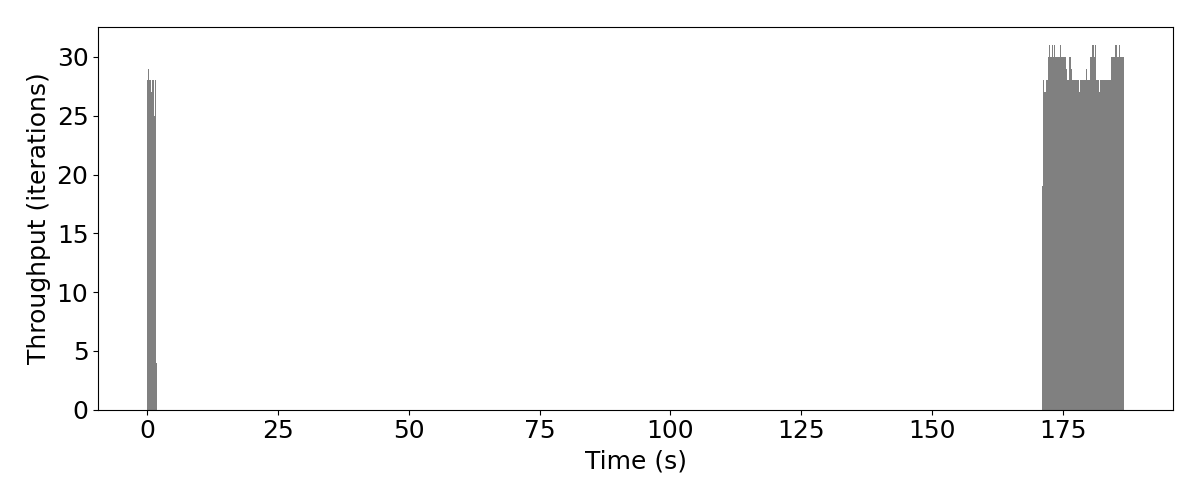
\includegraphics[width=\columnwidth]{graphs/parked-kubernetes.png}
    \caption{A \beclass{} process in a Kubernetes pod, parked while the
    antagonist runs and then resuming}\label{fig:parked-kubernetes}
\end{figure}

We investigate parking by running a BE Kubernetes pod alongside an antagonist,
and find that even after being parked for multiple minutes in the middle of
processing a request, the BE job is able to resume and return the final result
to the client. \autoref{fig:parked-kubernetes} shows the throughput over time of
an image resize job running in a BE container running as \schedbe{}. A couple
seconds after sending a request to the image resize pod, we start an entirely
CPU-bound antagonist on the same set of cores as the BE is running. We can see
that the image resize job is completely paused for about two and a half minutes,
until the antagonist is done running. The job then continues and completes. The
client connection did not experience any issues, even when setting the TCP
keepalive timeout to expire within duration the BE spent being parked.

\begin{figure}[t]
    \centering
    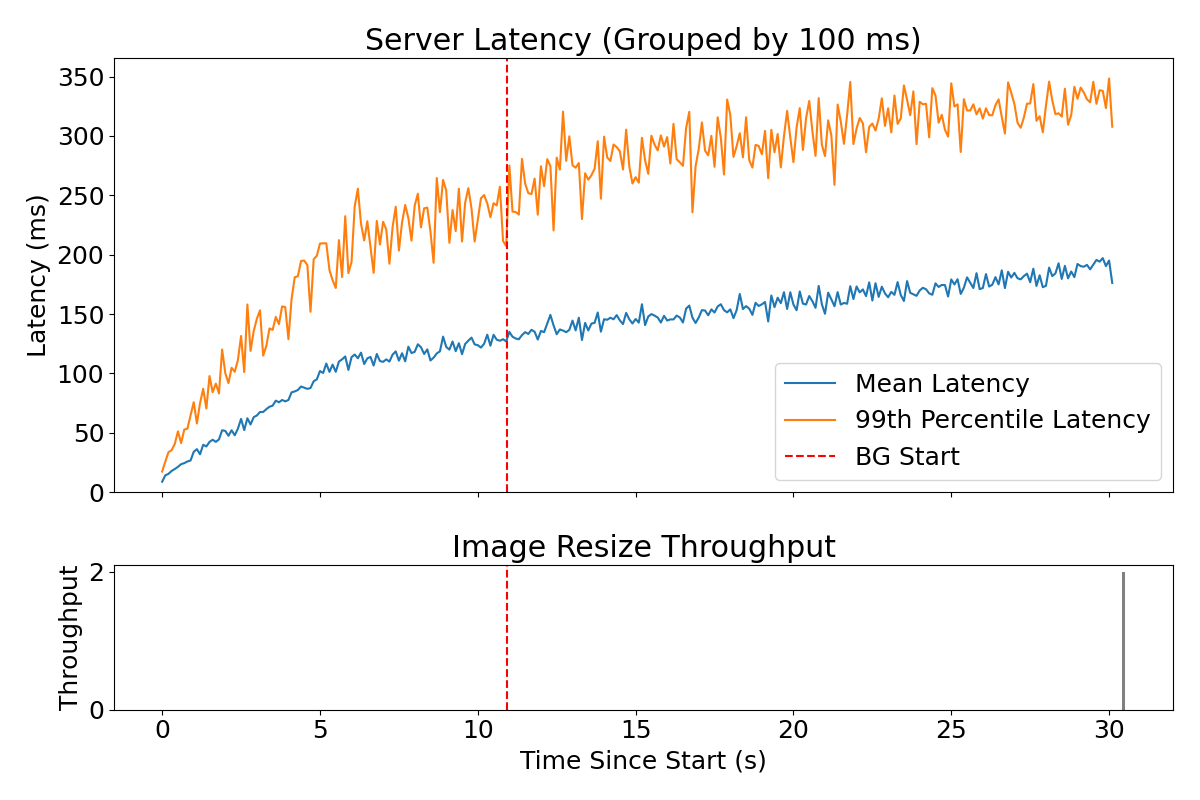
\includegraphics[width=\columnwidth]{graphs/overload-schedbe.png}
    \caption{BE in \schedbe{}, no throttling}\label{fig:overload-schedbe}
\end{figure}

\autoref{fig:overload-schedbe} shows how parking enables the LC to be isolated
from \schedbe{} even under sustained extremely high load. We run the same
experiment as \autoref{fig:overload-rt}, but now instead instead of throttling
the LC, the BE gets parked. Notice that the BE does not make progress until the
very end, when the server is done processing the requests. The difference is
stark: in both experiments, the open-loop client sent the same amount of
requests with the same amount of time in between them, but when the LC was
throttled it took the server 35s to process all the requests, with a final
latency of >1s, and with parking the server finished the client load in 31s with
a final avg latency of <200ms. 



\subsection{Cost of \schedbe{}}

The cost of \schedbe{} is can be broken down into the three checks that make up
the priority enforcement:

\begin{enumerate}
    \item \local{} adds a small amount of compute overhead on each scheduling
    decision to determine threads' priorities. This is a small amount of code we
    do not expect to impact latency
    \item \entry{} adds no new latency to Linux, which already implements
    \entry{} for \schedidle{}
    \item \exit{} adds overheads in two places: one is the cross-core check that
    each happens at each class boundary crossing, and the other is the overhead
    of the migration should it decide to steal a \schednormal{} process
\end{enumerate}

We look at how often the \exit{} check happens as well as how often it chooses
to steal in the Kubernetes experiment. The overhead of stealing the LC job is
known, and is a complicated function of the CPU architecture and which cores it
is moving between (\eg{} how much memory hierarchy do the two cores share).

% Please add the following required packages to your document preamble:
% \usepackage[normalem]{ulem}
% \useunder{\uline}{\ul}{}
\begin{table}[t]
    \centering
    \begin{tabular}{|l|l|l|}
        \hline
                & \# times runs & \# times successful \\ \hline
        \entry{} & $\sim$60K    & $\sim$12.5K         \\ \hline
        \exit{}  & $\sim$20K    & $\sim$10K          \\ \hline
    \end{tabular}
    \vspace{10pt}
    \caption{Counts of checks and how many times they run/are able to find an LC to
    run/a BE to interrupt}\label{tab:check-counts}
\end{table}

In the span of the 30 seconds the Kubernetes experiment takes to run, and across
the four cores it runs, we see the following: scheduling happens around 110K
times, which is a little less than once per ms on each core. The \entry{} check
happens $\sim$60K times, or about twice a ms. This makes sense: the client sends
a request every 2ms which will cause a server thread wakeup, and the software
stack includes Linux, Docker, and Kubernetes, all of which have worker threads.
Of those 60K \entry{} checks, 12.5K find an idle runqueue. The \exit{} check
happens fewer times, around 20K times, of which approximately half lead to
stealing a \schednormal{} task.

We can see that the \entry{} and \exit{} checks happen less than scheduling does
by more than half. This demonstrates that enforcing isolation between LC and BE
via priority classes requires much fewer cross-core checks than doing so at
every scheduling decision.

The other takeaway is that, under high load, the \exit{} check is effective:
around half of the time, the scheduler found a queued LC thread on another core.
Without the check, each of those would have led to a priority inversion.


\subsection{Comparison with \schedidle}\label{ss:eval:schedidle}

As discussed in \autoref{s:implementation}, \schedidle{} implements some but not
all of the isolation required of \beclass{}: it implements the \entry{} check,
but not the \exit{} check or strict local priorities.

\begin{figure}[t]
    \centering
    \begin{subfigure}[t]{\columnwidth}
        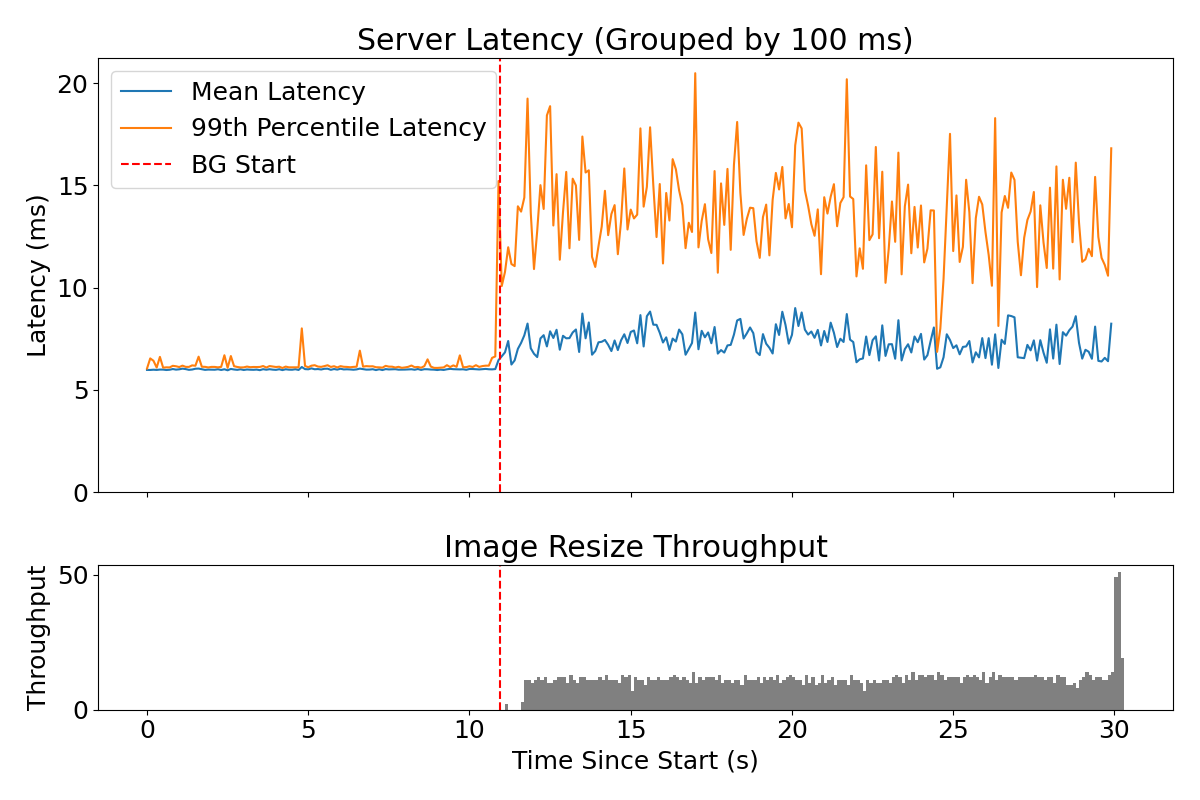
\includegraphics[width=\columnwidth]{graphs/srv-bg-idle-low.png}
        \caption{\schedidle{} in low load (85\%)}\label{fig:srv-bg-idle-low}
        \vspace{12pt}
    \end{subfigure}
    \hspace{\fill}
    \begin{subfigure}[t]{\columnwidth}
        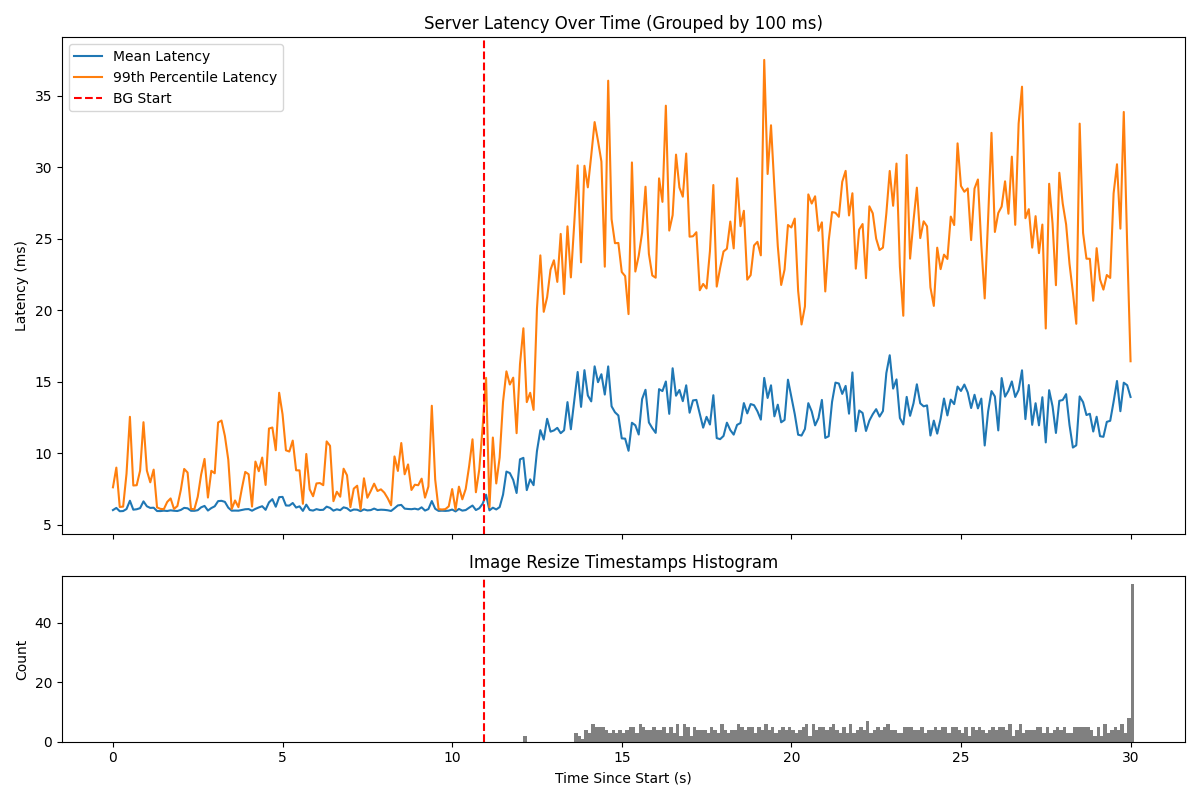
\includegraphics[width=\columnwidth]{graphs/srv-bg-idle-high.png}
        \caption{\schedidle{} in high load (95\%)}\label{fig:srv-bg-idle-high}
        \vspace{12pt}
    \end{subfigure}
    \hspace{\fill}
    \begin{subfigure}[t]{\columnwidth}
        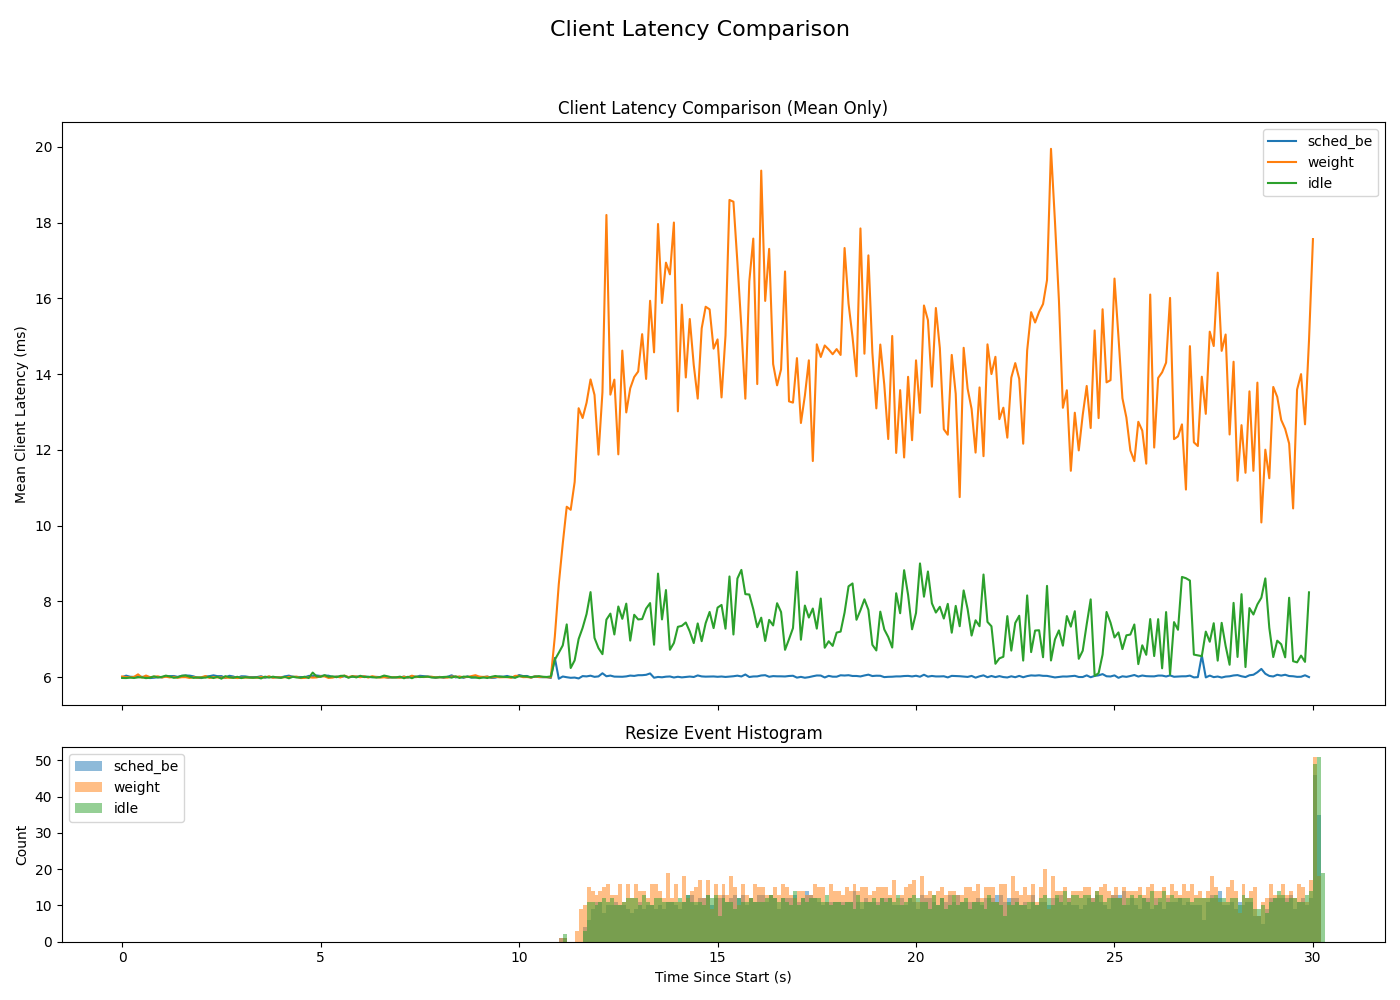
\includegraphics[width=\columnwidth]{graphs/srv-bg-cmp-all.png}
        \caption{Comparison of mean latency of the low load setting for weights,
        \schedidle{}, and \schedbe{}}\label{fig:srv-bg-cmp}
    \end{subfigure}
    \vspace{4pt}
    \caption{}\label{fig:srv-bg-idle}
\end{figure}

\begin{figure}[t]
    \centering
    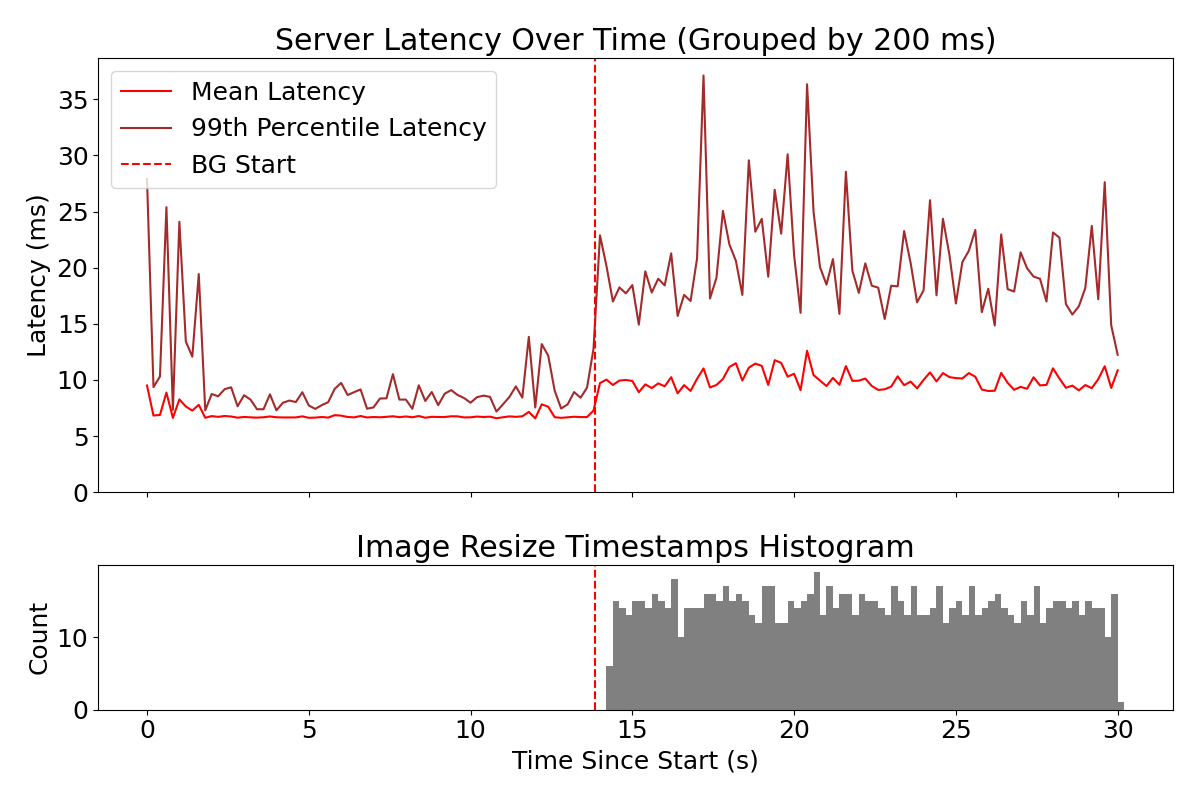
\includegraphics[width=\columnwidth]{graphs/kubernetes-idle.png}
    \caption{The same experiment as in \autoref{fig:kubernetes-unedited}, but
    running the BE as a \schedidle{} task}\label{fig:kubernetes-idle}
\end{figure}

\autoref{fig:srv-bg-idle} shows the result of running the BE jobs in the
microbenchmark in \schedidle{}, as well as a graph that compares the low load
setting of the standard \cgroups{} weight, \schedbe{}, and \schedidle{}. Average
latency still increases from $\sim$6ms to $\sim$8ms in the low load setting.
Although this increase is smaller than the original increase to $\sim$15ms using
the standard weight interface, it is still high compared to the 0ms increase
that \schedbe{} achieves. \autoref{fig:kubernetes-idle} shows similar results
for the Kubernetes experiment.
\section{Related work}

Some existing work focuses on isolating real-time applications in
Linux~\cite{rt-in-linux, state-rt-linux}, while Wasted Cores~\cite{wasted-cores}
focuses on the idle behavior of the Linux scheduler.

Other systems work around the kernel scheduler, by running primarily in
userspace~\cite{perfiso,caladan,skyloft}.

Linux's own \schedidle{} policy attempts to address this issue, but does not
fully solve it (running the microbenchmark using \schedidle{} still leads to an
increase in the mean latency from 6ms to 8).
%-------------------------------------------------------------------------------
\section{Conclusion}
%-------------------------------------------------------------------------------

This work shows that current isolation systems like Kubernetes are unable to
effectively performance isolate between LC and BE workloads for workloads that
are CPU-intensive. We trace this problem down to Linux's \cgroups{}, and show
that because Linux uses per-core runqueues, its weight-based interface for
isolation is not enforced across cores. Using a weight-based interface for
isolating LC and BE has other problems as well: it makes it hard to enforce a
split across cores, and it interacts poorly with the large scheduling quantum
that Linux uses.

Instead, we propose an API that separates BEs from LCs by introducing the
\beclass{} priority class. Enforcing \beclass{} requires less cross-core
interaction than a weight-based isolation approach, and ensures that no BE is
ever running when an LC is queued. During high load this requires `parking',
which enforces that BEs are immediately runnable once the load goes down, with
minimal interference for LCs in the meantime while the load is high.

We implement this strict priority in Linux, and show that the resulting
\schedbe{} allows \cgroups{} itself, as well as higher level applications that
build on \cgroups{} like Kubernetes, to do a better job of isolating LC from BE
workloads. Using \schedbe{} rather than the standard \cgroups{} weight interface
decrease the impact starting a BE process has on LC latencies from >2x to 0, and
under high load a parked \schedbe{} process running in a Kubernetes pod can
resume execution normally after multiple minutes of no user space CPU time.



%-------------------------------------------------------------------------------
%\bibliography{paper.bib}
\printbibliography

%%%%%%%%%%%%%%%%%%%%%%%%%%%%%%%%%%%%%%%%%%%%%%%%%%%%%%%%%%%%%%%%%%%%%%%%%%%%%%%%
\end{document}
%%%%%%%%%%%%%%%%%%%%%%%%%%%%%%%%%%%%%%%%%%%%%%%%%%%%%%%%%%%%%%%%%%%%%%%%%%%%%%%%

%%  LocalWords:  endnotes includegraphics fread ptr nobj noindent
%%  LocalWords:  pdflatex acks
